\documentclass{article}

\usepackage[main,final]{neurips_2025}
\usepackage{fontspec}
\setmainfont{texgyretermes}[Extension=.otf, UprightFont=*-regular, BoldFont=*-bold, ItalicFont=*-italic, BoldItalicFont=*-bolditalic]
\usepackage[brazil]{babel}
\usepackage{graphicx}
\usepackage{booktabs}
\usepackage{xcolor}
\usepackage{amsmath}
\usepackage{xspace}
\usepackage{hyperref}

% the final option prints a NeurIPS acceptance line, and this is a course paper
\makeatletter
\renewcommand{\@noticestring}{Trabalho final de disciplina, PPGCC, UFMG, 2026.}
\makeatother

\newcommand{\todo}[1]{\textcolor{red}{[TODO: #1]}}
\newcommand{\ci}[2]{[#1; #2]}

% generated by paper/build_numbers.py, do not edit
\newcommand{\gapQwenTwentySevenUjb}{\ensuremath{-}31,7\xspace}
\newcommand{\gapQwenTwentySevenUjbLo}{\ensuremath{-}40,5\xspace}
\newcommand{\gapQwenTwentySevenUjbHi}{\ensuremath{-}22,8\xspace}
\newcommand{\gapItemQwenTwentySevenUjbLo}{\ensuremath{-}37,8\xspace}
\newcommand{\gapItemQwenTwentySevenUjbHi}{\ensuremath{-}25,5\xspace}
\newcommand{\holmQwenTwentySevenUjb}{$1{,}0 \times 10^{-5}$\xspace}
\newcommand{\textRateQwenTwentySevenUjb}{54,0\xspace}
\newcommand{\tokenRatioQwenTwentySevenUjb}{0,47\xspace}
\newcommand{\contrastQwenTwentySevenUjb}{\ensuremath{-}4,05\xspace}
\newcommand{\contrastQwenTwentySevenUjbLo}{\ensuremath{-}4,81\xspace}
\newcommand{\contrastQwenTwentySevenUjbHi}{\ensuremath{-}3,29\xspace}
\newcommand{\gapGemmaTwelveUjb}{\ensuremath{-}36,2\xspace}
\newcommand{\gapGemmaTwelveUjbLo}{\ensuremath{-}44,4\xspace}
\newcommand{\gapGemmaTwelveUjbHi}{\ensuremath{-}28,1\xspace}
\newcommand{\gapItemGemmaTwelveUjbLo}{\ensuremath{-}44,1\xspace}
\newcommand{\gapItemGemmaTwelveUjbHi}{\ensuremath{-}28,4\xspace}
\newcommand{\holmGemmaTwelveUjb}{$1{,}1 \times 10^{-6}$\xspace}
\newcommand{\textRateGemmaTwelveUjb}{44,5\xspace}
\newcommand{\tokenRatioGemmaTwelveUjb}{0,18\xspace}
\newcommand{\contrastGemmaTwelveUjb}{\ensuremath{-}5,71\xspace}
\newcommand{\contrastGemmaTwelveUjbLo}{\ensuremath{-}6,63\xspace}
\newcommand{\contrastGemmaTwelveUjbHi}{\ensuremath{-}4,80\xspace}
\newcommand{\gapMistralTwentyFourUjb}{\ensuremath{-}31,1\xspace}
\newcommand{\gapMistralTwentyFourUjbLo}{\ensuremath{-}41,3\xspace}
\newcommand{\gapMistralTwentyFourUjbHi}{\ensuremath{-}20,9\xspace}
\newcommand{\gapItemMistralTwentyFourUjbLo}{\ensuremath{-}37,4\xspace}
\newcommand{\gapItemMistralTwentyFourUjbHi}{\ensuremath{-}24,7\xspace}
\newcommand{\holmMistralTwentyFourUjb}{$3{,}4 \times 10^{-5}$\xspace}
\newcommand{\textRateMistralTwentyFourUjb}{43,4\xspace}
\newcommand{\tokenRatioMistralTwentyFourUjb}{0,70\xspace}
\newcommand{\contrastMistralTwentyFourUjb}{\ensuremath{-}4,51\xspace}
\newcommand{\contrastMistralTwentyFourUjbLo}{\ensuremath{-}5,31\xspace}
\newcommand{\contrastMistralTwentyFourUjbHi}{\ensuremath{-}3,72\xspace}
\newcommand{\gapQwenNineUjb}{\ensuremath{-}28,9\xspace}
\newcommand{\gapQwenNineUjbLo}{\ensuremath{-}32,8\xspace}
\newcommand{\gapQwenNineUjbHi}{\ensuremath{-}25,0\xspace}
\newcommand{\gapItemQwenNineUjbLo}{\ensuremath{-}35,9\xspace}
\newcommand{\gapItemQwenNineUjbHi}{\ensuremath{-}21,9\xspace}
\newcommand{\holmQwenNineUjb}{$3{,}2 \times 10^{-9}$\xspace}
\newcommand{\textRateQwenNineUjb}{41,4\xspace}
\newcommand{\tokenRatioQwenNineUjb}{0,47\xspace}
\newcommand{\contrastQwenNineUjb}{\ensuremath{-}4,27\xspace}
\newcommand{\contrastQwenNineUjbLo}{\ensuremath{-}5,06\xspace}
\newcommand{\contrastQwenNineUjbHi}{\ensuremath{-}3,48\xspace}
\newcommand{\gapQwenVLSevenUjb}{\ensuremath{-}12,8\xspace}
\newcommand{\gapQwenVLSevenUjbLo}{\ensuremath{-}20,8\xspace}
\newcommand{\gapQwenVLSevenUjbHi}{\ensuremath{-}4,8\xspace}
\newcommand{\gapItemQwenVLSevenUjbLo}{\ensuremath{-}18,0\xspace}
\newcommand{\gapItemQwenVLSevenUjbHi}{\ensuremath{-}7,6\xspace}
\newcommand{\holmQwenVLSevenUjb}{0,0044\xspace}
\newcommand{\textRateQwenVLSevenUjb}{22,2\xspace}
\newcommand{\tokenRatioQwenVLSevenUjb}{0,66\xspace}
\newcommand{\contrastQwenVLSevenUjb}{\ensuremath{-}2,37\xspace}
\newcommand{\contrastQwenVLSevenUjbLo}{\ensuremath{-}3,14\xspace}
\newcommand{\contrastQwenVLSevenUjbHi}{\ensuremath{-}1,61\xspace}
\newcommand{\gapSonnetUjb}{\ensuremath{-}6,2\xspace}
\newcommand{\gapSonnetUjbLo}{\ensuremath{-}10,8\xspace}
\newcommand{\gapSonnetUjbHi}{\ensuremath{-}1,7\xspace}
\newcommand{\gapItemSonnetUjbLo}{\ensuremath{-}9,3\xspace}
\newcommand{\gapItemSonnetUjbHi}{\ensuremath{-}3,2\xspace}
\newcommand{\holmSonnetUjb}{0,032\xspace}
\newcommand{\textRateSonnetUjb}{97,4\xspace}
\newcommand{\tokenRatioSonnetUjb}{0,42\xspace}
\newcommand{\contrastSonnetUjb}{\ensuremath{-}3,08\xspace}
\newcommand{\contrastSonnetUjbLo}{\ensuremath{-}4,88\xspace}
\newcommand{\contrastSonnetUjbHi}{\ensuremath{-}1,27\xspace}
\newcommand{\gapOpusUjb}{\ensuremath{-}2,0\xspace}
\newcommand{\gapOpusUjbLo}{\ensuremath{-}3,7\xspace}
\newcommand{\gapOpusUjbHi}{\ensuremath{-}0,3\xspace}
\newcommand{\gapItemOpusUjbLo}{\ensuremath{-}4,3\xspace}
\newcommand{\gapItemOpusUjbHi}{0,4\xspace}
\newcommand{\holmOpusUjb}{0,040\xspace}
\newcommand{\textRateOpusUjb}{97,4\xspace}
\newcommand{\tokenRatioOpusUjb}{0,42\xspace}
\newcommand{\contrastOpusUjb}{\ensuremath{-}1,07\xspace}
\newcommand{\contrastOpusUjbLo}{\ensuremath{-}2,60\xspace}
\newcommand{\contrastOpusUjbHi}{0,46\xspace}
\newcommand{\gapQwenTwentySevenDev}{\ensuremath{-}27,9\xspace}
\newcommand{\gapQwenTwentySevenDevLo}{\ensuremath{-}32,0\xspace}
\newcommand{\gapQwenTwentySevenDevHi}{\ensuremath{-}23,7\xspace}
\newcommand{\gapItemQwenTwentySevenDevLo}{\ensuremath{-}30,6\xspace}
\newcommand{\gapItemQwenTwentySevenDevHi}{\ensuremath{-}25,2\xspace}
\newcommand{\holmQwenTwentySevenDev}{$9{,}1 \times 10^{-21}$\xspace}
\newcommand{\textRateQwenTwentySevenDev}{53,5\xspace}
\newcommand{\tokenRatioQwenTwentySevenDev}{0,47\xspace}
\newcommand{\contrastQwenTwentySevenDev}{\ensuremath{-}4,34\xspace}
\newcommand{\contrastQwenTwentySevenDevLo}{\ensuremath{-}4,69\xspace}
\newcommand{\contrastQwenTwentySevenDevHi}{\ensuremath{-}3,99\xspace}
\newcommand{\gapGemmaTwelveDev}{\ensuremath{-}30,3\xspace}
\newcommand{\gapGemmaTwelveDevLo}{\ensuremath{-}35,3\xspace}
\newcommand{\gapGemmaTwelveDevHi}{\ensuremath{-}25,3\xspace}
\newcommand{\gapItemGemmaTwelveDevLo}{\ensuremath{-}33,3\xspace}
\newcommand{\gapItemGemmaTwelveDevHi}{\ensuremath{-}27,3\xspace}
\newcommand{\holmGemmaTwelveDev}{$1{,}4 \times 10^{-18}$\xspace}
\newcommand{\textRateGemmaTwelveDev}{46,1\xspace}
\newcommand{\tokenRatioGemmaTwelveDev}{0,21\xspace}
\newcommand{\contrastGemmaTwelveDev}{\ensuremath{-}5,19\xspace}
\newcommand{\contrastGemmaTwelveDevLo}{\ensuremath{-}5,57\xspace}
\newcommand{\contrastGemmaTwelveDevHi}{\ensuremath{-}4,81\xspace}
\newcommand{\gapMistralTwentyFourDev}{\ensuremath{-}31,1\xspace}
\newcommand{\gapMistralTwentyFourDevLo}{\ensuremath{-}35,9\xspace}
\newcommand{\gapMistralTwentyFourDevHi}{\ensuremath{-}26,3\xspace}
\newcommand{\gapItemMistralTwentyFourDevLo}{\ensuremath{-}33,8\xspace}
\newcommand{\gapItemMistralTwentyFourDevHi}{\ensuremath{-}28,3\xspace}
\newcommand{\holmMistralTwentyFourDev}{$4{,}9 \times 10^{-20}$\xspace}
\newcommand{\textRateMistralTwentyFourDev}{48,3\xspace}
\newcommand{\tokenRatioMistralTwentyFourDev}{0,69\xspace}
\newcommand{\contrastMistralTwentyFourDev}{\ensuremath{-}4,95\xspace}
\newcommand{\contrastMistralTwentyFourDevLo}{\ensuremath{-}5,31\xspace}
\newcommand{\contrastMistralTwentyFourDevHi}{\ensuremath{-}4,59\xspace}
\newcommand{\gapQwenNineDev}{\ensuremath{-}23,4\xspace}
\newcommand{\gapQwenNineDevLo}{\ensuremath{-}27,8\xspace}
\newcommand{\gapQwenNineDevHi}{\ensuremath{-}19,0\xspace}
\newcommand{\gapItemQwenNineDevLo}{\ensuremath{-}25,9\xspace}
\newcommand{\gapItemQwenNineDevHi}{\ensuremath{-}20,9\xspace}
\newcommand{\holmQwenNineDev}{$6{,}2 \times 10^{-16}$\xspace}
\newcommand{\textRateQwenNineDev}{41,2\xspace}
\newcommand{\tokenRatioQwenNineDev}{0,47\xspace}
\newcommand{\contrastQwenNineDev}{\ensuremath{-}3,86\xspace}
\newcommand{\contrastQwenNineDevLo}{\ensuremath{-}4,20\xspace}
\newcommand{\contrastQwenNineDevHi}{\ensuremath{-}3,52\xspace}
\newcommand{\gapQwenVLSevenDev}{\ensuremath{-}16,4\xspace}
\newcommand{\gapQwenVLSevenDevLo}{\ensuremath{-}20,1\xspace}
\newcommand{\gapQwenVLSevenDevHi}{\ensuremath{-}12,7\xspace}
\newcommand{\gapItemQwenVLSevenDevLo}{\ensuremath{-}18,6\xspace}
\newcommand{\gapItemQwenVLSevenDevHi}{\ensuremath{-}14,1\xspace}
\newcommand{\holmQwenVLSevenDev}{$1{,}5 \times 10^{-12}$\xspace}
\newcommand{\textRateQwenVLSevenDev}{30,2\xspace}
\newcommand{\tokenRatioQwenVLSevenDev}{0,65\xspace}
\newcommand{\contrastQwenVLSevenDev}{\ensuremath{-}3,10\xspace}
\newcommand{\contrastQwenVLSevenDevLo}{\ensuremath{-}3,44\xspace}
\newcommand{\contrastQwenVLSevenDevHi}{\ensuremath{-}2,77\xspace}
\newcommand{\gapSonnetDev}{\ensuremath{-}6,1\xspace}
\newcommand{\gapSonnetDevLo}{\ensuremath{-}8,1\xspace}
\newcommand{\gapSonnetDevHi}{\ensuremath{-}4,2\xspace}
\newcommand{\gapItemSonnetDevLo}{\ensuremath{-}7,8\xspace}
\newcommand{\gapItemSonnetDevHi}{\ensuremath{-}4,4\xspace}
\newcommand{\holmSonnetDev}{$7{,}2 \times 10^{-8}$\xspace}
\newcommand{\textRateSonnetDev}{85,4\xspace}
\newcommand{\tokenRatioSonnetDev}{0,42\xspace}
\newcommand{\contrastSonnetDev}{\ensuremath{-}1,86\xspace}
\newcommand{\contrastSonnetDevLo}{\ensuremath{-}2,34\xspace}
\newcommand{\contrastSonnetDevHi}{\ensuremath{-}1,39\xspace}
\newcommand{\gapOpusDev}{\ensuremath{-}1,7\xspace}
\newcommand{\gapOpusDevLo}{\ensuremath{-}3,2\xspace}
\newcommand{\gapOpusDevHi}{\ensuremath{-}0,3\xspace}
\newcommand{\gapItemOpusDevLo}{\ensuremath{-}2,8\xspace}
\newcommand{\gapItemOpusDevHi}{\ensuremath{-}0,6\xspace}
\newcommand{\holmOpusDev}{0,040\xspace}
\newcommand{\textRateOpusDev}{92,8\xspace}
\newcommand{\tokenRatioOpusDev}{0,42\xspace}
\newcommand{\contrastOpusDev}{\ensuremath{-}0,74\xspace}
\newcommand{\contrastOpusDevLo}{\ensuremath{-}1,30\xspace}
\newcommand{\contrastOpusDevHi}{\ensuremath{-}0,18\xspace}
\newcommand{\nItemsUjb}{136\xspace}
\newcommand{\nClustersUjb}{14\xspace}
\newcommand{\gapMeanUjb}{\ensuremath{-}28,1\xspace}
\newcommand{\gapMeanUjbLo}{\ensuremath{-}33,2\xspace}
\newcommand{\gapMeanUjbHi}{\ensuremath{-}22,0\xspace}
\newcommand{\gapMinUjb}{\ensuremath{-}36,2\xspace}
\newcommand{\gapMaxUjb}{\ensuremath{-}12,8\xspace}
\newcommand{\tokenRatioMinUjb}{0,18\xspace}
\newcommand{\tokenRatioMaxUjb}{0,70\xspace}
\newcommand{\holmMaxUjb}{0,0044\xspace}
\newcommand{\nItemsDev}{859\xspace}
\newcommand{\nClustersDev}{79\xspace}
\newcommand{\gapMeanDev}{\ensuremath{-}25,8\xspace}
\newcommand{\gapMeanDevLo}{\ensuremath{-}29,7\xspace}
\newcommand{\gapMeanDevHi}{\ensuremath{-}21,7\xspace}
\newcommand{\gapMinDev}{\ensuremath{-}31,1\xspace}
\newcommand{\gapMaxDev}{\ensuremath{-}16,4\xspace}
\newcommand{\tokenRatioMinDev}{0,21\xspace}
\newcommand{\tokenRatioMaxDev}{0,69\xspace}
\newcommand{\holmMaxDev}{$1{,}5 \times 10^{-12}$\xspace}
\newcommand{\tokenRatioMinAll}{0,18\xspace}
\newcommand{\tokenRatioMaxAll}{0,70\xspace}
\newcommand{\holmMaxAll}{0,0044\xspace}
\newcommand{\claudeLossMinAll}{1,7\xspace}
\newcommand{\claudeLossMaxAll}{6,2\xspace}
\newcommand{\sdItemConditionUjb}{0,91\xspace}
\newcommand{\sdItemConditionUjbLo}{0,60\xspace}
\newcommand{\sdItemConditionUjbHi}{1,21\xspace}
\newcommand{\sdItemUjb}{3,44\xspace}
\newcommand{\sdRatioUjb}{0,26\xspace}
\newcommand{\sdRatioProbitUjb}{0,29\xspace}
\newcommand{\waldStatUjb}{40,1\xspace}
\newcommand{\waldDfUjb}{4\xspace}
\newcommand{\waldPUjb}{$4{,}0 \times 10^{-8}$\xspace}
\newcommand{\lrtStatUjb}{14,1\xspace}
\newcommand{\lrtPUjb}{$8{,}9 \times 10^{-5}$\xspace}
\newcommand{\heldoutDiffUjb}{4,8\xspace}
\newcommand{\heldoutSeUjb}{5,1\xspace}
\newcommand{\heldoutPositiveFoldsUjb}{7\xspace}
\newcommand{\heldoutFoldsUjb}{10\xspace}
\newcommand{\bhFlaggedUjb}{0\xspace}
\newcommand{\rawFlaggedUjb}{1\xspace}
\newcommand{\nItemFlagsUjb}{544\xspace}
\newcommand{\corrTenUjb}{0,62\xspace}
\newcommand{\corrTenUjbRefLo}{0,64\xspace}
\newcommand{\corrTenUjbRefHi}{0,78\xspace}
\newcommand{\slopeTenUjb}{0,31\xspace}
\newcommand{\slopeCorrectedTenUjb}{0,36\xspace}
\newcommand{\corrTwelveUjb}{0,66\xspace}
\newcommand{\corrTwelveUjbRefLo}{0,67\xspace}
\newcommand{\corrTwelveUjbRefHi}{0,81\xspace}
\newcommand{\slopeTwelveUjb}{0,35\xspace}
\newcommand{\slopeCorrectedTwelveUjb}{0,41\xspace}
\newcommand{\corrFourteenUjb}{0,75\xspace}
\newcommand{\corrFourteenUjbRefLo}{0,71\xspace}
\newcommand{\corrFourteenUjbRefHi}{0,83\xspace}
\newcommand{\slopeFourteenUjb}{0,46\xspace}
\newcommand{\slopeCorrectedFourteenUjb}{0,53\xspace}
\newcommand{\slopeTextRunCorrUjb}{0,86\xspace}
\newcommand{\cPearsonUjb}{0,14\xspace}
\newcommand{\cPearsonRefLoUjb}{0,01\xspace}
\newcommand{\cPearsonRefHiUjb}{0,11\xspace}
\newcommand{\cPearsonPercentileUjb}{99,7\xspace}
\newcommand{\sdItemConditionDev}{1,39\xspace}
\newcommand{\sdItemConditionDevLo}{1,27\xspace}
\newcommand{\sdItemConditionDevHi}{1,51\xspace}
\newcommand{\sdItemDev}{4,45\xspace}
\newcommand{\sdRatioDev}{0,31\xspace}
\newcommand{\sdRatioProbitDev}{0,33\xspace}
\newcommand{\waldStatDev}{126,9\xspace}
\newcommand{\waldDfDev}{4\xspace}
\newcommand{\waldPDev}{$1{,}8 \times 10^{-26}$\xspace}
\newcommand{\lrtStatDev}{321,8\xspace}
\newcommand{\lrtPDev}{$2{,}9 \times 10^{-72}$\xspace}
\newcommand{\heldoutDiffDev}{182,2\xspace}
\newcommand{\heldoutSeDev}{46,6\xspace}
\newcommand{\heldoutPositiveFoldsDev}{10\xspace}
\newcommand{\heldoutFoldsDev}{10\xspace}
\newcommand{\bhFlaggedDev}{0\xspace}
\newcommand{\rawFlaggedDev}{38\xspace}
\newcommand{\nItemFlagsDev}{3436\xspace}
\newcommand{\corrTenDev}{0,59\xspace}
\newcommand{\corrTenDevRefLo}{0,74\xspace}
\newcommand{\corrTenDevRefHi}{0,79\xspace}
\newcommand{\slopeTenDev}{0,39\xspace}
\newcommand{\slopeCorrectedTenDev}{0,42\xspace}
\newcommand{\corrTwelveDev}{0,65\xspace}
\newcommand{\corrTwelveDevRefLo}{0,77\xspace}
\newcommand{\corrTwelveDevRefHi}{0,82\xspace}
\newcommand{\slopeTwelveDev}{0,44\xspace}
\newcommand{\slopeCorrectedTwelveDev}{0,48\xspace}
\newcommand{\corrFourteenDev}{0,74\xspace}
\newcommand{\corrFourteenDevRefLo}{0,81\xspace}
\newcommand{\corrFourteenDevRefHi}{0,85\xspace}
\newcommand{\slopeFourteenDev}{0,52\xspace}
\newcommand{\slopeCorrectedFourteenDev}{0,56\xspace}
\newcommand{\slopeTextRunCorrDev}{0,93\xspace}
\newcommand{\cPearsonDev}{0,22\xspace}
\newcommand{\cPearsonRefLoDev}{0,08\xspace}
\newcommand{\cPearsonRefHiDev}{0,11\xspace}
\newcommand{\cPearsonPercentileDev}{100,0\xspace}
\newcommand{\floorTextQwenVLSevenUjb}{68,4\xspace}
\newcommand{\floorTenQwenVLSevenUjb}{88,2\xspace}
\newcommand{\floorTwelveQwenVLSevenUjb}{85,3\xspace}
\newcommand{\floorFourteenQwenVLSevenUjb}{85,3\xspace}
\newcommand{\noPassTextUjb}{23,5\xspace}
\newcommand{\allPassTextUjb}{8,8\xspace}
\newcommand{\noPassImageMinUjb}{52,2\xspace}
\newcommand{\noPassImageMaxUjb}{62,5\xspace}
\newcommand{\sizeDiffMinUjb}{8,8\xspace}
\newcommand{\sizeDiffMaxUjb}{8,8\xspace}
\newcommand{\lopoMinUjb}{\ensuremath{-}38,4\xspace}
\newcommand{\lopoMaxUjb}{\ensuremath{-}12,3\xspace}
\newcommand{\floorTextQwenVLSevenDev}{62,2\xspace}
\newcommand{\floorTenQwenVLSevenDev}{82,8\xspace}
\newcommand{\floorTwelveQwenVLSevenDev}{80,1\xspace}
\newcommand{\floorFourteenQwenVLSevenDev}{78,8\xspace}
\newcommand{\noPassTextDev}{31,4\xspace}
\newcommand{\allPassTextDev}{15,0\xspace}
\newcommand{\noPassImageMinDev}{51,3\xspace}
\newcommand{\noPassImageMaxDev}{63,6\xspace}
\newcommand{\sizeDiffMinDev}{4,1\xspace}
\newcommand{\sizeDiffMaxDev}{6,3\xspace}
\newcommand{\flaggedGapMinUjb}{\ensuremath{-}77,3\xspace}
\newcommand{\flaggedGapMaxUjb}{\ensuremath{-}32,7\xspace}
\newcommand{\copiedItemsUjb}{25\xspace}
\newcommand{\controlHighModelsUjb}{3\xspace}
\newcommand{\flagBothMinUjb}{2\xspace}
\newcommand{\flagBothMaxUjb}{4\xspace}
\newcommand{\copiedItemsClaudeUjb}{128\xspace}
\newcommand{\flaggedSonnetUjb}{126\xspace}
\newcommand{\unflaggedSonnetUjb}{10\xspace}
\newcommand{\flaggedOpusUjb}{106\xspace}
\newcommand{\unflaggedOpusUjb}{30\xspace}
\newcommand{\flaggedGapMinDev}{\ensuremath{-}64,1\xspace}
\newcommand{\flaggedGapMaxDev}{\ensuremath{-}35,0\xspace}
\newcommand{\copiedItemsDev}{149\xspace}
\newcommand{\controlHighModelsDev}{3\xspace}
\newcommand{\flagBothMinDev}{14\xspace}
\newcommand{\flagBothMaxDev}{27\xspace}
\newcommand{\copiedItemsClaudeDev}{706\xspace}
\newcommand{\flaggedSonnetDev}{673\xspace}
\newcommand{\unflaggedSonnetDev}{186\xspace}
\newcommand{\flaggedOpusDev}{492\xspace}
\newcommand{\unflaggedOpusDev}{367\xspace}
\newcommand{\contamGaps}{40\xspace}
\newcommand{\contamShrinking}{39\xspace}
\newcommand{\indentShareUjb}{17,3\xspace}
\newcommand{\relOneTextUjb}{0,68\xspace}
\newcommand{\relTwoTextUjb}{0,81\xspace}
\newcommand{\gFiniteTextUjb}{0,94\xspace}
\newcommand{\gFiniteTextUjbLo}{0,86\xspace}
\newcommand{\gFiniteTextUjbHi}{0,97\xspace}
\newcommand{\relOneTenUjb}{0,62\xspace}
\newcommand{\relTwoTenUjb}{0,77\xspace}
\newcommand{\gFiniteTenUjb}{0,85\xspace}
\newcommand{\gFiniteTenUjbLo}{0,49\xspace}
\newcommand{\gFiniteTenUjbHi}{0,93\xspace}
\newcommand{\relOneTwelveUjb}{0,63\xspace}
\newcommand{\relTwoTwelveUjb}{0,77\xspace}
\newcommand{\gFiniteTwelveUjb}{0,61\xspace}
\newcommand{\gFiniteTwelveUjbLo}{0,01\xspace}
\newcommand{\gFiniteTwelveUjbHi}{0,86\xspace}
\newcommand{\relOneFourteenUjb}{0,59\xspace}
\newcommand{\relTwoFourteenUjb}{0,74\xspace}
\newcommand{\gFiniteFourteenUjb}{0,92\xspace}
\newcommand{\gFiniteFourteenUjbLo}{0,80\xspace}
\newcommand{\gFiniteFourteenUjbHi}{0,95\xspace}
\newcommand{\indentShareDev}{18,4\xspace}
\newcommand{\relOneTextDev}{0,76\xspace}
\newcommand{\relTwoTextDev}{0,86\xspace}
\newcommand{\gFiniteTextDev}{0,98\xspace}
\newcommand{\gFiniteTextDevLo}{0,97\xspace}
\newcommand{\gFiniteTextDevHi}{0,99\xspace}
\newcommand{\relOneTenDev}{0,70\xspace}
\newcommand{\relTwoTenDev}{0,82\xspace}
\newcommand{\gFiniteTenDev}{0,92\xspace}
\newcommand{\gFiniteTenDevLo}{0,84\xspace}
\newcommand{\gFiniteTenDevHi}{0,95\xspace}
\newcommand{\relOneTwelveDev}{0,68\xspace}
\newcommand{\relTwoTwelveDev}{0,81\xspace}
\newcommand{\gFiniteTwelveDev}{0,94\xspace}
\newcommand{\gFiniteTwelveDevLo}{0,90\xspace}
\newcommand{\gFiniteTwelveDevHi}{0,97\xspace}
\newcommand{\relOneFourteenDev}{0,67\xspace}
\newcommand{\relTwoFourteenDev}{0,80\xspace}
\newcommand{\gFiniteFourteenDev}{0,95\xspace}
\newcommand{\gFiniteFourteenDevLo}{0,92\xspace}
\newcommand{\gFiniteFourteenDevHi}{0,97\xspace}
\newcommand{\harnessSuspects}{13\xspace}
\newcommand{\harnessUnpassable}{12\xspace}
\newcommand{\handReadAnswers}{40\xspace}
\newcommand{\neverPassedChecked}{10\xspace}
\newcommand{\bootReps}{2000\xspace}
\newcommand{\glmmTmbVersion}{1.1.14\xspace}
\newcommand{\rVersion}{4.5.3\xspace}
\newcommand{\neverPassedAllSeven}{18\xspace}
\newcommand{\neverPassedTestBug}{9\xspace}
\newcommand{\handReadFalseFails}{2\xspace}
\newcommand{\handReadOf}{40\xspace}
\newcommand{\handReadPct}{5,0\xspace}
\newcommand{\handReadCiLo}{0,6\xspace}
\newcommand{\handReadCiHi}{16,9\xspace}
\newcommand{\checklistYes}{6\xspace}
\newcommand{\checklistPartly}{9\xspace}
\newcommand{\checklistNo}{4\xspace}
\newcommand{\checklistNA}{4\xspace}
\newcommand{\harnessShrinkPct}{1,4\xspace}
\newcommand{\underspecifiedItems}{3\xspace}
\newcommand{\underspecifiedOf}{10\xspace}
\newcommand{\nameErrorGrowthPoints}{23\xspace}
\newcommand{\nameErrorNearCopies}{400\xspace}
\newcommand{\sizeDiffMinAll}{4,1\xspace}
\newcommand{\sizeDiffMaxAll}{8,8\xspace}
\newcommand{\relOneMinUjb}{0,59\xspace}
\newcommand{\relOneMaxUjb}{0,68\xspace}
\newcommand{\relTwoMinUjb}{0,74\xspace}
\newcommand{\relTwoMaxUjb}{0,81\xspace}
\newcommand{\relThreeMinUjb}{0,81\xspace}
\newcommand{\relThreeMaxUjb}{0,86\xspace}
\newcommand{\gFiniteMinUjb}{0,85\xspace}
\newcommand{\gFiniteMaxUjb}{0,94\xspace}
\newcommand{\swapGemmaQwenNineUjb}{0,79\xspace}
\newcommand{\corrBelowRefUjb}{2\xspace}
\newcommand{\ceilingTextSonnetUjb}{97,1\xspace}
\newcommand{\ceilingTextOpusUjb}{95,6\xspace}
\newcommand{\relOneMinDev}{0,67\xspace}
\newcommand{\relOneMaxDev}{0,76\xspace}
\newcommand{\relTwoMinDev}{0,80\xspace}
\newcommand{\relTwoMaxDev}{0,86\xspace}
\newcommand{\relThreeMinDev}{0,86\xspace}
\newcommand{\relThreeMaxDev}{0,90\xspace}
\newcommand{\gFiniteMinDev}{0,92\xspace}
\newcommand{\gFiniteMaxDev}{0,98\xspace}
\newcommand{\swapGemmaQwenNineDev}{0,98\xspace}
\newcommand{\corrBelowRefDev}{3\xspace}
\newcommand{\ceilingTextSonnetDev}{82,9\xspace}
\newcommand{\ceilingTextOpusDev}{89,9\xspace}
\newcommand{\claudeTemperature}{1,0\xspace}
\newcommand{\openClosedCUjb}{2,75\xspace}
\newcommand{\openClosedCUjbLo}{1,40\xspace}
\newcommand{\openClosedCUjbHi}{4,10\xspace}
\newcommand{\openClosedCDev}{3,85\xspace}
\newcommand{\openClosedCDevLo}{3,39\xspace}
\newcommand{\openClosedCDevHi}{4,31\xspace}
\newcommand{\blockOneItemsDev}{200\xspace}
\newcommand{\blockOneItemsUjb}{40\xspace}
\newcommand{\blockOneLossMin}{9\xspace}
\newcommand{\blockOneLossMax}{39\xspace}
\newcommand{\lengthGapShort}{13\xspace}
\newcommand{\lengthGapLong}{26\xspace}
\newcommand{\nameErrorTextNearCopies}{2\xspace}
\newcommand{\pilotProblems}{20\xspace}
\newcommand{\pilotTextPass}{60\xspace}
\newcommand{\pilotImagePass}{60\xspace}
\newcommand{\pilotOf}{100\xspace}
\newcommand{\nameDevText}{8\xspace}
\newcommand{\nameDevImage}{31\xspace}
\newcommand{\nameUjbText}{17\xspace}
\newcommand{\nameUjbImage}{40\xspace}


\title{Código como imagem: quanto modelos de visão e linguagem perdem ao ler o contexto do repositório em pixels}

\author{%
  Carlos Henrique Brito Malta Leão \\
  Programa de Pós-Graduação em Ciência da Computação \\
  Universidade Federal de Minas Gerais \\
  \texttt{chbmleao@ufmg.br}
}

\begin{document}

\maketitle

\begin{abstract}
Renderizar o contexto de um repositório como imagem reduz os tokens de entrada, mas não se sabe quanto isso custa em código que precisa passar em testes. Medimos esse custo em cinco modelos abertos de visão e linguagem, de 7B a 27B, em \nItemsAll itens do CoderUJB (Java) e do DevEval (Python), com o contexto em texto e em imagem a 10, 12 e 14 px. Os cinco modelos abertos passam menos testes com a imagem. O gap médio dos modelos, imagem menos texto, é \gapMeanUjb~pp \ci{\gapMeanUjbLo}{\gapMeanUjbHi} no CoderUJB e \gapMeanDev~pp \ci{\gapMeanDevLo}{\gapMeanDevHi} no DevEval. Por modelo, o gap vai de \gapMinUjb{} a \gapMaxUjb~pp e de \gapMinDev{} a \gapMaxDev~pp, e a razão de tokens de entrada vai de \tokenRatioMinAll{} a \tokenRatioMaxAll. Como resultado secundário, a penalidade varia entre itens (DP item:condição de \sdItemConditionUjb{} e \sdItemConditionDev{} em logit), mas no CoderUJB a comparação fora da amostra não apoia essa variação. Em uma extensão exploratória, o Claude Sonnet 5.5 e o Opus 5.5 também perdem, de \claudeLossMinAll{} a \claudeLossMaxAll~pp.
\end{abstract}

\section{Introdução}
Modelos de visão e linguagem (VLMs) leem texto renderizado como imagem, e isso abre uma forma de comprimir o contexto. O DeepSeek-OCR decodifica com cerca de 97\% de precisão abaixo de 10x de compressão \citep{wei2025deepseekocr}, o Glyph usa a ideia em contexto longo \citep{cheng2025glyph} e o CodeOCR a leva para código \citep{shi2026codeocr}. Em nossos dados, o contexto em imagem usa de \tokenRatioMinAll{} a \tokenRatioMaxAll{} dos tokens de entrada do texto. Falta saber quanto isso custa quando o código gerado precisa passar em testes.

A lacuna está no tipo de avaliação. \citet{liang2026rendered} corrigem com testes no nível de repositório, mas com um agente, 100 tarefas do SWE-bench Verified e uma execução por célula. Sem agente, nenhum trabalho que encontramos corrige a geração no nível de repositório com testes de unidade, nenhum avalia o Gemma 4 nem o Mistral Small 3.2, e nenhum testa com um modelo de efeitos mistos se o gap varia entre modelos e entre itens (Seção~\ref{sec:penalidade}).

Neste trabalho a renderização é uma intervenção que nós atribuímos: cada item aparece nas quatro condições, em cada modelo, e a resposta é a aprovação nos testes do próprio benchmark. A matriz de respostas pareada \citep[Seção~2.5]{truong2026measurement} dá o gap de cada modelo com intervalo agrupado por projeto ou repositório (Seção~\ref{sec:gap}). Um GLMM com a condição como faceta \citep[cap.~3]{truong2026measurement} separa a variância do item da variância do item por condição (Seção~\ref{sec:penalidade}). O construto é estreito, completar uma função ou um método com o contexto do repositório, e os limites vêm na Seção~\ref{sec:limit}.

As contribuições são três. Primeiro, o gap por modelo, de \gapMinUjb{} a \gapMaxUjb~pp no CoderUJB e de \gapMinDev{} a \gapMaxDev~pp no DevEval, com intervalos. Segundo, uma penalidade que não é igual entre itens no DevEval, com apoio mais fraco no CoderUJB e sem identificar itens individuais. Terceiro, um argumento de validade que reporta todos os desvios do plano.

\section{Trabalhos relacionados}
% 1. Texto renderizado em VLMs: Reading Not Thinking, VISTA-Bench, ReadBench, PixelWorld.
\todo{texto renderizado em VLMs}
% 2. Compressão por imagem e código: VisInContext, VIST, DeepSeek-OCR, CodeOCR, LongCodeOCR, CodeShrink e o estudo do ComplexCodeEval. Nenhum avalia no nível de repositório com testes.
\todo{compressão por imagem e código}
% 3. Estatística de avaliação: intervalos agrupados (Miller) e poucos itens (Bowyer); variância entre execuções (Madaan, Bouthillier); contaminação (Ramos, Riddell); não há testes de heterogeneidade.
\todo{estatística de avaliação}

\section{Métodos}

\subsection{Dados}
% CoderUJB: itens, projetos e o Defects4J usado para corrigir (n_items, n_clusters); DevEval: itens e repositórios; filtros (2k a 12k tokens, a referência passa); licenças (benchmarks/README.md, tabela Licenses).
\todo{CoderUJB, DevEval, filtros e licenças}

\subsection{Modelos e condições}
% Os 5 modelos, a precisão e o vLLM; renderização compacta em JetBrains Mono a 10, 12 e 14 px, páginas de 616 x 1540; tarefa em texto e contexto em imagem; 2 ou 3 execuções por célula, temperatura 0,7, sem thinking (methodology 3.1).
\todo{modelos, renderização e execuções}

\subsection{Construto e estimandos}
% O construto e o que fica fora dele; delta_mb como efeito total do pacote de renderização (livro cap. 9, nível 2), sem ajuste por tokens (methodology 3.2).
\todo{construto e estimando}

\subsection{Análise}
% IC CR1 agrupado, Holm nos 10 gaps, média dos modelos por reamostragem conjunta (gaps settings).
\todo{intervalos, Holm e média dos modelos}
% GLMM: fórmula, glmmTMB, R; checagens de uma habilidade (correlações, inclinação comum, probit, log-verossimilhança fora da amostra); flag de contaminação com controle pareado; confiabilidade por MCMC.
\todo{GLMM, checagens de uma habilidade, contaminação e confiabilidade}

\subsection{Desvios do pré-registro}
% Desvios que tocam as afirmações principais, com data: 2 ou 3 execuções por célula (2026-11-10); Wald no lugar do LRT e Laplace no lugar de Monte Carlo (2026-11-16); transcrição como bônus, leitura manual no Sonnet com 10 por condição, checagem de 10 dos 18 itens que ninguém passa e os 12 itens suspeitos mantidos (2026-11-23). O resto vai para a Tabela A1.
\todo{desvios principais com data, e remissão à Tabela A1}
\todo{UFM-33: decisão sobre os 12 itens do DevEval. Fallback: os 12 ficam e contam como falha, com efeito de cerca de 1,4 por cento}
\todo{UFM-34: leitura manual com rótulos checados. Fallback: a leitura manual cobre só o Sonnet}
\todo{UFM-28: transcrição, leitura contra programação. Fallback: planejado e não concluído, citando o desvio de 2026-11-23}

\section{Resultados}

\subsection{Gap por modelo}
% Os 10 gaps são negativos, com IC abaixo de 0 (asserção em build_numbers), e o maior p de Holm; média dos modelos (pooled).
\todo{gaps por modelo, IC e maior p de Holm}
% Tabela 1 (gerada): por modelo e benchmark, taxa em texto, gap [IC], contraste logit [IC] e razão de tokens.
\todo{leitura da Tabela 1}
% Leitura ordinal por causa do piso, com o Qwen2.5-VL (floor_ceiling); leave-one-project-out no CoderUJB, numa frase (lopo).
\todo{piso e leave-one-project-out}

\begin{figure}[t]
  \centering
  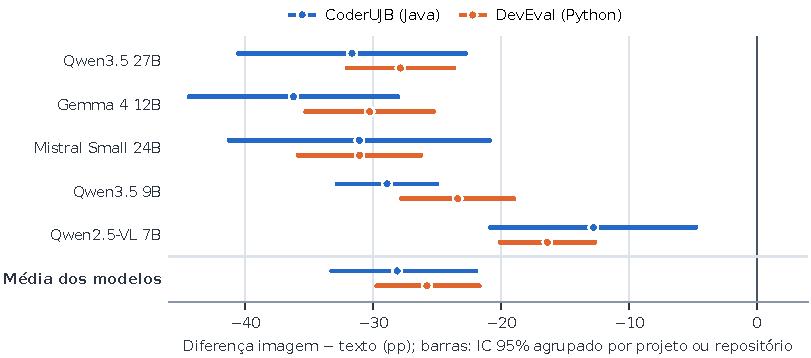
\includegraphics[width=\linewidth]{figures/fig_gap}
  \caption{\todo{legenda da Figura 1: gap imagem menos texto por modelo aberto e média dos modelos, IC 95\% agrupado por projeto}}
  \label{fig:gap}
\end{figure}

\begin{table}[t]
  \centering
  \caption{\todo{legenda da Tabela 1}}
  \label{tab:gaps}
  \resizebox{\linewidth}{!}{\begin{tabular}{lrrcrcr}
\toprule
Modelo & Texto (\%) & Gap (pp) & IC 95\% & Contraste (logit) & IC 95\% & Razão de tokens \\
\midrule
\multicolumn{7}{l}{\emph{CoderUJB, 136 itens}} \\
Qwen3.5 27B & 54,0 & \ensuremath{-}31,7 & [\ensuremath{-}40,5; \ensuremath{-}22,8] & \ensuremath{-}4,05 & [\ensuremath{-}4,81; \ensuremath{-}3,29] & 0,47 \\
Gemma 4 12B & 44,5 & \ensuremath{-}36,2 & [\ensuremath{-}44,4; \ensuremath{-}28,1] & \ensuremath{-}5,71 & [\ensuremath{-}6,63; \ensuremath{-}4,80] & 0,18 \\
Mistral Small 3.2 24B & 43,4 & \ensuremath{-}31,1 & [\ensuremath{-}41,3; \ensuremath{-}20,9] & \ensuremath{-}4,51 & [\ensuremath{-}5,31; \ensuremath{-}3,72] & 0,70 \\
Qwen3.5 9B & 41,4 & \ensuremath{-}28,9 & [\ensuremath{-}32,8; \ensuremath{-}25,0] & \ensuremath{-}4,27 & [\ensuremath{-}5,06; \ensuremath{-}3,48] & 0,47 \\
Qwen2.5-VL 7B & 22,2 & \ensuremath{-}12,8 & [\ensuremath{-}20,8; \ensuremath{-}4,8] & \ensuremath{-}2,37 & [\ensuremath{-}3,14; \ensuremath{-}1,61] & 0,66 \\
\emph{Média dos modelos} &  & \ensuremath{-}28,1 & [\ensuremath{-}33,2; \ensuremath{-}22,0] &  &  &  \\
\midrule
\multicolumn{7}{l}{\emph{DevEval, 859 itens}} \\
Qwen3.5 27B & 53,5 & \ensuremath{-}27,9 & [\ensuremath{-}32,0; \ensuremath{-}23,7] & \ensuremath{-}4,34 & [\ensuremath{-}4,69; \ensuremath{-}3,99] & 0,47 \\
Gemma 4 12B & 46,1 & \ensuremath{-}30,3 & [\ensuremath{-}35,3; \ensuremath{-}25,3] & \ensuremath{-}5,19 & [\ensuremath{-}5,57; \ensuremath{-}4,81] & 0,21 \\
Mistral Small 3.2 24B & 48,3 & \ensuremath{-}31,1 & [\ensuremath{-}35,9; \ensuremath{-}26,3] & \ensuremath{-}4,95 & [\ensuremath{-}5,31; \ensuremath{-}4,59] & 0,69 \\
Qwen3.5 9B & 41,2 & \ensuremath{-}23,4 & [\ensuremath{-}27,8; \ensuremath{-}19,0] & \ensuremath{-}3,86 & [\ensuremath{-}4,20; \ensuremath{-}3,52] & 0,47 \\
Qwen2.5-VL 7B & 30,2 & \ensuremath{-}16,4 & [\ensuremath{-}20,1; \ensuremath{-}12,7] & \ensuremath{-}3,10 & [\ensuremath{-}3,44; \ensuremath{-}2,77] & 0,65 \\
\emph{Média dos modelos} &  & \ensuremath{-}25,8 & [\ensuremath{-}29,7; \ensuremath{-}21,7] &  &  &  \\
\bottomrule
\end{tabular}
}
\end{table}

\subsection{Fonte e tokens}
% 14 px supera 12 px por 4,1 a 8,8 pp, com IC acima de 0, para o Qwen3.5 27B nos dois benchmarks e para o Mistral e o Qwen3.5 9B no DevEval (size_diffs; asserção sobre o conjunto); o Gemma economiza mais tokens e perde o mesmo em todo tamanho.
\todo{efeito do tamanho da fonte e economia de tokens}

\begin{figure}[t]
  \centering
  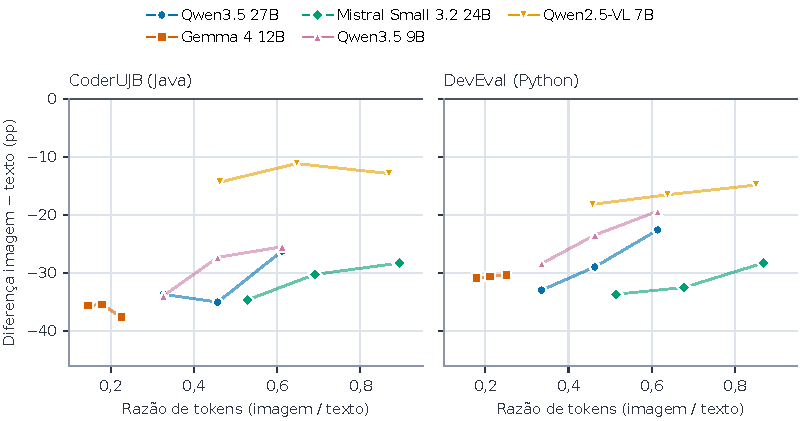
\includegraphics[width=\linewidth]{figures/fig_size_tokens}
  \caption{\todo{legenda da Figura 2: gap por tamanho contra a razão de tokens por tamanho, uma linha por modelo}}
  \label{fig:size-tokens}
\end{figure}

\subsection{A penalidade é igual entre itens e modelos?}
% Wald com 4 gl; DP item:condição com IC de perfil e razão sobre o DP de item; LRT como linha secundária; log-verossimilhança fora da amostra, positiva nas 10 dobras no DevEval e indistinguível de 0 no CoderUJB (asserção).
\todo{Wald, DP item:condição, LRT e fora da amostra}
% Correlação texto x imagem abaixo da referência e C de Pearson nos percentis 0,997 e 1,000; inclinação comum dividida por r e probit; nenhum item sobrevive ao BH (asserção); com 5 modelos não se estabelece uma segunda habilidade.
\todo{correlações, inclinação comum, probit, BH e limite de 5 modelos}

\begin{figure}[t]
  \centering
  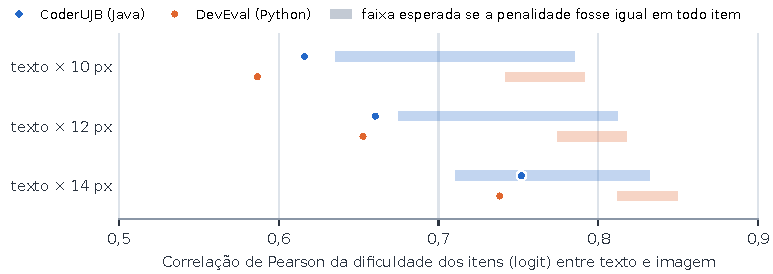
\includegraphics[width=\linewidth]{figures/fig_item_corr}
  \caption{\todo{legenda da Figura 3: correlação texto x imagem por tamanho contra a faixa de referência}}
  \label{fig:item-corr}
\end{figure}

\subsection{Confiabilidade e ordem}
% Confiabilidade de 1 e de 2 execuções e o G finito; CoderUJB a 12 px é instável; os três modelos do meio trocam de lugar (reliability.json; docs/paper/reliability.md como rascunho).
\todo{confiabilidade, G finito e troca de ordem}

\subsection{Contaminação}
% 25 e 149 itens com cópia (copied_items); 39 de 40 gaps encolhem e todos seguem negativos; controle acima do percentil 97,5 em 3 de 5 modelos por benchmark; os itens marcados perdem mais (associação e checagem fora do plano); concordância das duas flags (flag2).
\todo{contaminação: cópias, encolhimento, controle, itens marcados e flags}

\subsection{Exploratório}
% Claude perde de 1,7 a 6,2 pp; contraste c; teto no CoderUJB; itens marcados (claude main, glmm, contamination). Marcar como exploratório.
\todo{Claude, exploratório}
% Bloco 1: os erros a mais são de nome, com o exemplo _determine_alterations; o piloto não teve gap (block1/findings.md). Marcar como exploratório.
\todo{bloco 1, exploratório}

\section{Discussão}

\subsection{Argumento de validade}
\label{sec:validade}
Seguimos as cinco evidências de \citealp[seç.~1.2]{truong2026measurement}. A evidência de construto é a principal: a renderização é atribuída por desenho a todo modelo e item, o resto fica fixo, e o gap é esse contraste. Ela não mostra por que a imagem perde, porque modalidade, tokens e layout mudam juntos. A de conteúdo é parcial: o construto é uma função ou método com contexto de repositório, não programar em geral, e o conteúdo dos itens não foi auditado por inteiro. A de critério é parcial: o texto serve de critério concorrente, e a dificuldade dos itens em texto e em imagem tem correlação moderada (Fig.~\ref{fig:item-corr}), mas os testes unitários são o desfecho, não um critério independente. A externa é limitada (Seção~\ref{sec:limit}). A consequencial não foi estudada. Pelo checklist de \citealp[seç.~13.5]{truong2026measurement}, \checklistYes{} são atendidos, \checklistPartly{} em parte, \checklistNo{} não e \checklistNA{} não se aplicam. Em termos causais (cap.~9), só o gap é um contraste intervencional. A contaminação, o comprimento e os erros de nome são associações, e não afirmamos que causem a perda.

\subsection{Sensibilidade à fonte: validade ou confiabilidade?}
\label{sec:disc-fonte}
O exercício 1.5 \#1 pergunta se a sensibilidade ao tamanho da fonte é um problema de validade ou de confiabilidade. O efeito de 14 px sobre 12 px em alguns pares (Seção~\ref{sec:fonte}) é sistemático: repetir a mesma condição mais vezes reduz o ruído entre execuções, mas não o move. Como o tamanho da fonte não faz parte do construto, é variância irrelevante ao construto \citep[seç.~1.3]{truong2026measurement}, uma ameaça à validade. Ela só viraria faceta de confiabilidade se o tamanho fosse amostrado de uma população de tamanhos num estudo G.

\subsection{Contaminação ou variância irrelevante ao construto?}
\label{sec:disc-contam}
O exercício 1.5 \#3 pede para separar os dois casos. Chamamos de contaminação um caminho que contorna a habilidade: o modelo reproduz a referência por tê-la visto, e isso depende do item e do modelo. O contraste pareado cancela esse caminho se ele afeta texto e imagem do mesmo jeito. Não cancela se ele interage com a modalidade, por exemplo se a cópia for mais fácil de acionar em texto. Os itens marcados perdem mais com a imagem (Seção~\ref{sec:contam}), o que é compatível com essa interação, mas é uma associação fora do plano, e há outra leitura: nesses itens os modelos passam mais em texto e têm mais a perder. No nosso caso, portanto, é contaminação, e ela só vira variância irrelevante ao construto do contraste se interagir com a modalidade.

\subsection{Quando o DIF é um problema a corrigir}
\label{sec:disc-dif}
O exercício 1.5 \#5 pergunta quando o funcionamento diferencial do item (DIF, \citealp[seç.~5.11]{truong2026measurement}) pede correção. Aqui o DIF é a interação item:condição, não uma comparação entre grupos de modelos. Corrige-se quando a fonte é irrelevante ao construto, como um corretor que falha em certos itens só no caminho de uma condição; os \excludedDev{} itens do DevEval cuja referência o nosso corretor não deixa passar eram falha do corretor em toda condição e foram excluídos em 25/11/2026. O layout não é DIF: age sobre a condição inteira e entra como variância irrelevante ao construto (Seção~\ref{sec:disc-fonte}). Reporta-se quando a variação pode refletir ler o contexto, o que não medimos. Essa variação é pouco estabelecida: fora da amostra ela se sustenta no DevEval, e no CoderUJB não.

\subsection{Teste de transferência}
\label{sec:transferencia}
Pelo cap.~11 de \citet{truong2026measurement}, o avaliador só é durável se o resultado se mantém fora das condições do estudo. A replicação entre benchmarks, com o gap abaixo de zero nos dois, já foi observada e não conta como previsão. Fixamos duas previsões antes de qualquer nova rodada. (i) Com um renderizador sem indentação, que libera cerca de \indentShareUjb{}\% e \indentShareDev{}\% dos caracteres, o intervalo do gap médio dos modelos abertos segue abaixo de zero; a previsão é refutada se ele incluir zero, o que atribuiria a perda ao layout. (ii) Os itens cuja transcrição do contexto tem erro passam menos em imagem que os de transcrição fiel; a previsão é refutada se o intervalo dessa diferença incluir zero. Um resultado a favor seria compatível com erro de leitura, sem separar leitura de programação. Nenhuma das duas foi testada: o renderizador não foi rodado, e a transcrição não foi concluída (Seção~\ref{sec:desvios}).

\section{Limitações}
% 1. Modelos: 5 abertos, de 7B a 27B. O Claude é exploratório (temperatura 1,0, sem seed): mesma direção, perda menor.
\todo{limitação 1: modelos}
% 2. Um único renderizador: a indentação é 17,3 e 18,4 por cento dos caracteres e não foi testada. Parágrafo do CodeShrink (layout.json; results/layout/findings.md).
\todo{limitação 2: um renderizador e a indentação}
% 3. Sem baseline sem contexto: a UFM-29 foi cancelada, e o CodeOCR mostra um modelo abaixo do baseline.
\todo{limitação 3: sem baseline sem contexto}
% 4. Contaminação e teto (copied_items; claude flagged).
\todo{limitação 4: contaminação e teto}
% 5. Evidência por item e leitura x programação: nenhum item sobrevive ao BH; leitura manual de 40 respostas do Sonnet, com rótulos não checados por pessoa; leitura x programação não foi medida; a única evidência de erro de leitura é a contagem do bloco 1.
\todo{limitação 5: evidência por item e leitura contra programação}
\todo{UFM-34: rótulos da leitura manual checados por pessoa}
\todo{UFM-28: leitura contra programação medida pela transcrição}
% 6. Itens e construto: 12 itens do DevEval provavelmente impassáveis, cerca de 1,4 por cento de cada gap; 3 de 10 itens subespecificados; piso de 51 a 64 por cento; construto estreito e itens estáticos; G de 0,61 no CoderUJB a 12 px.
\todo{limitação 6: itens e construto}
\todo{UFM-33: efeito dos 12 itens do DevEval}

\section{Conclusão e trabalhos futuros}
Com o contexto em imagem, os cinco modelos abertos passam menos testes: \gapMeanUjb~pp na média do CoderUJB e \gapMeanDev~pp na do DevEval, para uma entrada de \tokenRatioMinAll{} a \tokenRatioMaxAll{} dos tokens do texto. O valor é deste renderizador e deste construto, e o Claude, exploratório, perde menos. Faltam medir a transcrição, renderizar sem indentação, incluir um baseline sem contexto e rodar mais modelos.
\label{body-end}


\bibliographystyle{plainnat}
\bibliography{refs}

\appendix
\setcounter{table}{0}
\setcounter{figure}{0}
\renewcommand{\thetable}{A\arabic{table}}
\renewcommand{\thefigure}{A\arabic{figure}}

\section{Desvios do pré-registro}
\label{app:deviations}
% A1: todos os desvios com data (decisions.md). Inclui: inclinação dividida por r, saída em tokens e gaps só dos itens marcados (2026-11-16); confiabilidade na escala 0/1 com termos de projeto (2026-11-14); desvios do Claude: sem seed, temperatura 1,0, Opus sempre pensa, regra over_budget, 2 execuções por orçamento, pesos fechados (2026-11-14); regra de descarte, regra da célula curta não construída, razão pela mediana (2026-11-17); layout só com os passos 1 e 5 (2026-11-17); exclusão dos \excludedDev itens do DevEval cuja referência não passa no corretor (2026-11-25); e os desvios da seção 3.5.
\todo{Tabela A1: todos os desvios com data (tabela escrita à mão)}

\section{Gaps por tamanho}
\label{app:sizes}
% A2: gaps por tamanho e diferenças entre tamanhos (sizes, size_diffs).
\begin{table}[h]
  \centering
  \caption{\todo{legenda da Tabela A2a: gap por tamanho, pp, IC 95\% agrupado}}
  \label{tab:sizes}
  \resizebox{\linewidth}{!}{\begin{tabular}{lccc}
\toprule
Modelo & 10 px & 12 px & 14 px \\
\midrule
\multicolumn{4}{l}{\emph{CoderUJB}} \\
Qwen3.5 27B & \ensuremath{-}33,7 [\ensuremath{-}40,8; \ensuremath{-}26,6] & \ensuremath{-}35,0 [\ensuremath{-}45,3; \ensuremath{-}24,8] & \ensuremath{-}26,2 [\ensuremath{-}35,9; \ensuremath{-}16,5] \\
Gemma 4 12B & \ensuremath{-}35,7 [\ensuremath{-}43,9; \ensuremath{-}27,4] & \ensuremath{-}35,4 [\ensuremath{-}43,0; \ensuremath{-}27,9] & \ensuremath{-}37,6 [\ensuremath{-}46,9; \ensuremath{-}28,4] \\
Mistral Small 3.2 24B & \ensuremath{-}34,7 [\ensuremath{-}45,8; \ensuremath{-}23,5] & \ensuremath{-}30,3 [\ensuremath{-}40,8; \ensuremath{-}19,7] & \ensuremath{-}28,3 [\ensuremath{-}39,4; \ensuremath{-}17,2] \\
Qwen3.5 9B & \ensuremath{-}33,9 [\ensuremath{-}41,2; \ensuremath{-}26,7] & \ensuremath{-}27,3 [\ensuremath{-}31,0; \ensuremath{-}23,6] & \ensuremath{-}25,5 [\ensuremath{-}29,8; \ensuremath{-}21,2] \\
Qwen2.5-VL 7B & \ensuremath{-}14,3 [\ensuremath{-}24,7; \ensuremath{-}4,0] & \ensuremath{-}11,2 [\ensuremath{-}18,3; \ensuremath{-}4,0] & \ensuremath{-}12,9 [\ensuremath{-}21,0; \ensuremath{-}4,7] \\
\midrule
\multicolumn{4}{l}{\emph{DevEval}} \\
Qwen3.5 27B & \ensuremath{-}33,0 [\ensuremath{-}37,8; \ensuremath{-}28,1] & \ensuremath{-}29,0 [\ensuremath{-}33,7; \ensuremath{-}24,3] & \ensuremath{-}22,6 [\ensuremath{-}25,9; \ensuremath{-}19,3] \\
Gemma 4 12B & \ensuremath{-}30,9 [\ensuremath{-}35,5; \ensuremath{-}26,3] & \ensuremath{-}30,6 [\ensuremath{-}36,0; \ensuremath{-}25,3] & \ensuremath{-}30,4 [\ensuremath{-}35,4; \ensuremath{-}25,4] \\
Mistral Small 3.2 24B & \ensuremath{-}33,7 [\ensuremath{-}38,6; \ensuremath{-}28,8] & \ensuremath{-}32,5 [\ensuremath{-}37,3; \ensuremath{-}27,7] & \ensuremath{-}28,3 [\ensuremath{-}32,6; \ensuremath{-}23,9] \\
Qwen3.5 9B & \ensuremath{-}28,4 [\ensuremath{-}33,3; \ensuremath{-}23,5] & \ensuremath{-}23,5 [\ensuremath{-}28,2; \ensuremath{-}18,8] & \ensuremath{-}19,4 [\ensuremath{-}22,9; \ensuremath{-}15,8] \\
Qwen2.5-VL 7B & \ensuremath{-}18,2 [\ensuremath{-}22,5; \ensuremath{-}13,8] & \ensuremath{-}16,5 [\ensuremath{-}20,1; \ensuremath{-}12,9] & \ensuremath{-}14,8 [\ensuremath{-}18,3; \ensuremath{-}11,3] \\
\bottomrule
\end{tabular}
}
\end{table}
\begin{table}[h]
  \centering
  \caption{\todo{legenda da Tabela A2b: diferenças entre tamanhos, pp, IC 95\% agrupado}}
  \label{tab:size-diffs}
  \resizebox{\linewidth}{!}{\begin{tabular}{lccc}
\toprule
Modelo & 12 \ensuremath{-} 10 px & 14 \ensuremath{-} 10 px & 14 \ensuremath{-} 12 px \\
\midrule
\multicolumn{4}{l}{\emph{CoderUJB}} \\
Qwen3.5 27B & \ensuremath{-}1,3 [\ensuremath{-}5,3; 2,6] & 7,5 [4,0; 10,9] & 8,8 [5,2; 12,4] \\
Gemma 4 12B & 0,2 [\ensuremath{-}1,2; 1,7] & \ensuremath{-}2,0 [\ensuremath{-}6,1; 2,2] & \ensuremath{-}2,2 [\ensuremath{-}6,3; 1,8] \\
Mistral Small 3.2 24B & 4,4 [\ensuremath{-}1,2; 10,0] & 6,4 [\ensuremath{-}2,1; 14,8] & 2,0 [\ensuremath{-}4,7; 8,6] \\
Qwen3.5 9B & 6,6 [1,2; 12,0] & 8,5 [0,6; 16,3] & 1,8 [\ensuremath{-}2,9; 6,6] \\
Qwen2.5-VL 7B & 3,2 [\ensuremath{-}3,2; 9,5] & 1,5 [\ensuremath{-}4,9; 7,8] & \ensuremath{-}1,7 [\ensuremath{-}4,7; 1,3] \\
\midrule
\multicolumn{4}{l}{\emph{DevEval}} \\
Qwen3.5 27B & 3,9 [2,4; 5,5] & 10,2 [7,3; 13,2] & 6,3 [3,5; 9,1] \\
Gemma 4 12B & 0,2 [\ensuremath{-}1,5; 1,9] & 0,5 [\ensuremath{-}1,3; 2,2] & 0,3 [\ensuremath{-}1,2; 1,7] \\
Mistral Small 3.2 24B & 1,2 [\ensuremath{-}0,4; 2,7] & 5,3 [3,2; 7,4] & 4,2 [2,4; 5,9] \\
Qwen3.5 9B & 4,9 [3,1; 6,6] & 8,9 [6,3; 11,5] & 4,1 [1,8; 6,3] \\
Qwen2.5-VL 7B & 1,6 [0,0; 3,3] & 3,3 [1,5; 5,1] & 1,7 [\ensuremath{-}0,1; 3,5] \\
\bottomrule
\end{tabular}
}
\end{table}

\section{Correlação da dificuldade entre condições}
\label{app:item-corr}
\begin{figure}[h]
  \centering
  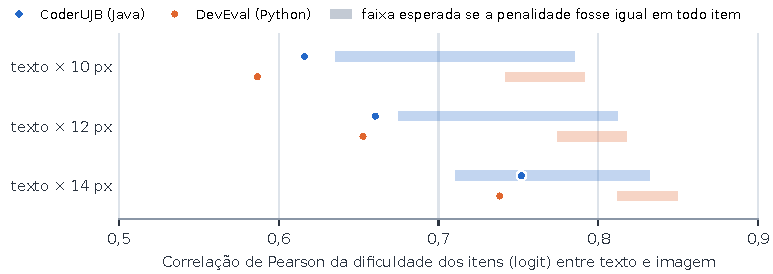
\includegraphics[width=\linewidth]{figures/fig_item_corr}
  \caption{Correlação de Pearson da dificuldade dos itens, em logit, entre texto e cada tamanho de imagem. Os pontos são os valores observados e a faixa clara é o intervalo de 2,5\% a 97,5\% simulado para uma penalidade igual em todo item. Pontos abaixo da faixa indicam que texto e imagem concordam menos do que esse caso prevê.}
  \label{fig:item-corr}
\end{figure}

\section{Análises secundárias do plano}
\label{app:secondary}
% A3: uma linha por análise: comprimento, scoring, lopo (length, scoring, lopo).
\todo{Tabela A3: análises secundárias do plano, uma linha cada}

\section{Claude, exploratório}
\label{app:claude}
% A4: tabela e figura do Claude (claude gaps).
\begin{table}[h]
  \centering
  \caption{\todo{legenda da Tabela A4: Claude, exploratório}}
  \label{tab:claude}
  \resizebox{\linewidth}{!}{\begin{tabular}{lrrcrcr}
\toprule
Modelo & Texto (\%) & Gap (pp) & IC 95\% & Contraste (logit) & IC 95\% & Razão de tokens \\
\midrule
\multicolumn{7}{l}{\emph{CoderUJB, 136 itens}} \\
Claude Sonnet 5.5 & 97,4 & \ensuremath{-}6,2 & [\ensuremath{-}10,8; \ensuremath{-}1,7] & \ensuremath{-}3,08 & [\ensuremath{-}4,88; \ensuremath{-}1,27] & 0,42 \\
Claude Opus 5.5 & 97,4 & \ensuremath{-}2,0 & [\ensuremath{-}3,7; \ensuremath{-}0,3] & \ensuremath{-}1,07 & [\ensuremath{-}2,60; 0,46] & 0,42 \\
\midrule
\multicolumn{7}{l}{\emph{DevEval, 859 itens}} \\
Claude Sonnet 5.5 & 85,4 & \ensuremath{-}6,1 & [\ensuremath{-}8,1; \ensuremath{-}4,2] & \ensuremath{-}1,86 & [\ensuremath{-}2,34; \ensuremath{-}1,39] & 0,42 \\
Claude Opus 5.5 & 92,8 & \ensuremath{-}1,7 & [\ensuremath{-}3,2; \ensuremath{-}0,3] & \ensuremath{-}0,74 & [\ensuremath{-}1,30; \ensuremath{-}0,18] & 0,42 \\
\bottomrule
\end{tabular}
}
\end{table}
\todo{figura do Claude}

\section{Contaminação}
\label{app:contamination}
% A5: tabela de contaminação (contamination.json).
\todo{Tabela A5: contaminação}


\end{document}
